\section{Entradas flotantes en compuertas TTL y CMOS}
\vspace{5mm}
Se implementaron los siguientes circuitos:

\begin{figure}[H]
    \begin{minipage}{.49\linewidth}
        \centering
        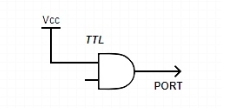
\includegraphics[width=.6\linewidth]{./TTLFlotante.jpg}
        \caption{Compuerta AND TTL con entrada flotante.}
        \label{fig:TTLFlotante}
    \end{minipage}
    \begin{minipage}{.5\linewidth}
        \centering
        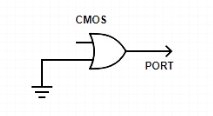
\includegraphics[width=.5\linewidth]{./CMOSFlotante.jpg}
        \caption{Compuerta OR CMOS con entrada flotante.}
        \label{fig:CMOSFlotante}
    \end{minipage}
\end{figure}

En primer lugar, en el caso de la compuerta TTL se conectó una entrada a Vcc (5V) y se dejó la otra flotante (figura \ref{fig:TTLFlotante}),
 es decir no se le realizó ninguna conexión y se midió la salida, que se observó constante como un 1 lógico (aproximadamente 5V). \\
En el caso de la CMOS, se dejó también un input flotante y otro se lo conectó a masa, como se ve en la figura \ref{fig:CMOSFlotante}. 
Se observó en este caso ruido de línea de 50Hz, con amplitud que variaba entre 0-0.8V, que no se encontraba entre las tensiones high y low de salida 
del CMOS ($V_{OH}~y~V_{OL}$)\footnote{Datos sacados de la datasheet: ver figura \ref{fig:cmos-threshold}.},
 es decir, la salida era indefinida (no era ni un 1 ni un 0 lógico). 

\begin{figure}[H]
    \centering
    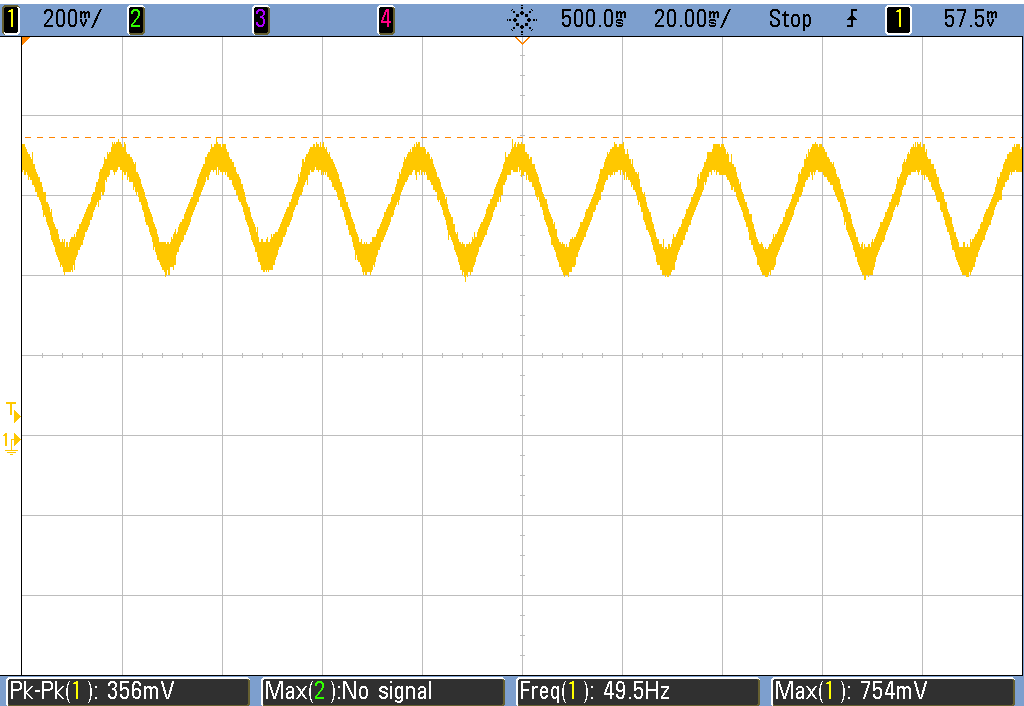
\includegraphics[width=.5\linewidth]{./ruidoCMOS.png}
    \caption{Ruido observado del CMOS con entrada flotante.}
    \label{fig:ruidoCMOS}
\end{figure}

\vspace{20mm}
\begin{wraptable}{l}{6.5cm}
    \begin{center}
        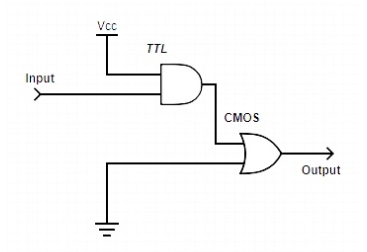
\includegraphics[scale=0.5]{./circuito.jpg}
        \caption{Circuito implementado.}
        \label{fig:circuito}
    \end{center}
\end{wraptable} 
\par
Para el CMOS este comportamiento puede deberse a que tiene alta impedancia de entrada por lo que al dejar una entrada flotante
funciona como antena, induciéndose corrientes, por ejemplo, por ruido, lo que genera tensiones a la entrada de la compuerta
ocasionando un nivel de tensión high o low incierto a la salida.
Para que no ocurra ésto, el fabricante recomienda conectar las entradas que no se utilizan ya sea a GND o a Vcc, 
para evitar estados operacionales indefinidos.\footnote{Referirse a la hoja de datos del fabricante: \url{http://www.ti.com/lit/ds/symlink/sn54hc32-sp.pdf}.}\\\newline

A continuación se implementó el circuito del cuadro \ref{fig:circuito}. No se observó ningún comportamiento indeseado, 
sin embargo, si se observan las figuras \ref{fig:ttl-threshold} y \ref{fig:cmos-threshold} que muestran los niveles de tensión high y low de entrada y salida 
para una compuerta TTL y CMOS ($V_{IH}/V_{IL}~~y~~V_{OH}/V_{OL}$), se pueden encontrar problemas si, por ejemplo, 
la tensión de entrada al circuito es de 3V; ésto ocasionaría que la salida de la TTL estuviera entre los 2.4V-5V para un 1 lógico, 
que podría presentar cierta incompatibilidad con los valores de tensión de entrada de la CMOS, ya que podría caer dentro de la zona indefinida, 
resultando en una salida incierta del circuito.\\
Posibles soluciones a este inconveniente serían utilizar mismas familias de compuertas, es decir, ambas TTL (LS) o CMOS (HC), lo que corrige estas ambigüedades.
Se implementó el nuevo circuito y no se encontraron problemas, como era esperable.

\begin{figure}[H]
    \begin{minipage}{.49\linewidth}
        \centering
       % \includegraphics[width=.6\linewidth]{./.jpg}
        \caption{Tensiones $V_{OH}, V_{OL}, V_{IH}, V_{IL} para una compuerta AND TTL.$}
        \label{fig:ttl-threshold}
    \end{minipage}
    \begin{minipage}{.5\linewidth}
        \centering
        %\includegraphics[width=.5\linewidth]{./.jpg}
        \caption{Tensiones $V_{OH}, V_{OL}, V_{IH}, V_{IL} para una compuerta OR CMOS.$}
        \label{fig:cmos-threshold}
    \end{minipage}
\end{figure}


A modo de síntesis, una entrada flotante en un TTL es considerada como un 1 lógico a la entrada, y un input flotante en CMOS tiene un comportamiento incierto
a la salida. Si bien, el circuito combinado con compuertas TTL y CMOS funciona de manera correcta, los fabricantes \textit{Texas Instruments}
\footnote{Nota de aplicación del fabricante:
Haseloff, E. (1997). Designing with Logic. \textit{Texas Instruments}, 6-7. Extraído de \url{http://www.ti.com/lit/an/sdya009c/sdya009c.pdf}.} 
y \textit{Fairchild} 
\footnote{Nota de aplicación del fabricante:
(1984). Application Note 363. Designing with TTL. \textit{Fairchild}, 2. Extraído de \url{https://www.fairchildsemi.com/application-notes/AN/AN-363.pdf}.} 
no pueden asegurar el valor de salida del integrado y recomiendan conectar todos los inputs sin utilizar a un valor de tensión conocido, sea GND, Vcc o cortocircuitarla con otra entrada que esté en uso, dependiendo de la función del circuito.
